\section{Simulation}

\subsection{Methodology}

As the simulation is not limited by hardware, all executions are able to run to completion. All simulations were run with the following parameters (similarly exaggerated to accelerate decay):

\begin{itemize}
    \item Blockchain
    \begin{itemize}
        \item Block reward - 12.5
        \item Global hash rate - 1
        \item Block time - 1
        \item Discount factor - 0.001\%
    \end{itemize}
    \item Pool 
    \begin{itemize}
        \item Hash rate - 0.3 (i.e. 30\%)
        \item Tax rate - 5\%
        \item Trade interval - 0.5
    \end{itemize}
    \item Participants
    \begin{itemize}
        \item Count - 3
        \item Initial chunks - 0
    \end{itemize}
    \item Reward minimum threshold - 0.009
\end{itemize}

\subsection{Results}

Figures \ref{figure:simulation-balance} and \ref{figure:simulation-chunks} are the results of a simulation with three participants, four chunks, and limited to 200 rounds. Figure \ref{figure:simulation-balance} below shows that the general trend is fairly balanced in the beginning but begins to diverge as balances increase. While participant 3 lags behind, this can be explained by the their reduced activity as seen in \cref{figure:simulation-chunks}. Despite this, the average distribution of funds observe a positive trend given the right conditions and do not diverge significantly.

\begin{figure}[H]
  \centering
  \caption{Balance distribution over shortened simulation lifespan}
  \label{figure:simulation-balance}
  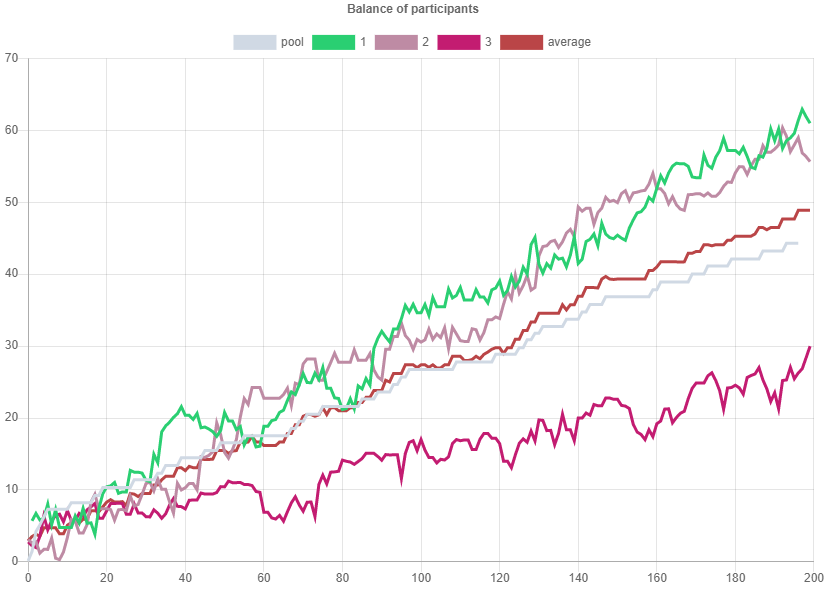
\includegraphics[width=0.8\textwidth]{media/simulation-balance.PNG}
\end{figure}

As seen in \cref{figure:simulation-chunks} below, the transition of funds occurred fairly frequently, effectively reducing any chance a participant may have in holding all the chunks. It is noted that there were several instances when a participant was able to hold all the chunks. while they were never in a participants possession for longer than a single round, it is less than ideal as it is possible for the game to reach such a state. Despite these spikes, the balances did not experience any sudden jumps in correlation to the possession of all chunks. This is likely due to the trade interval being half that of the block time, meaning a participant will likely have to maintain possession of the chunk for two rounds. 

\begin{figure}[H]
  \centering
  \caption{Chunk distribution over shortened simulation lifespan}
  \label{figure:simulation-chunks}
  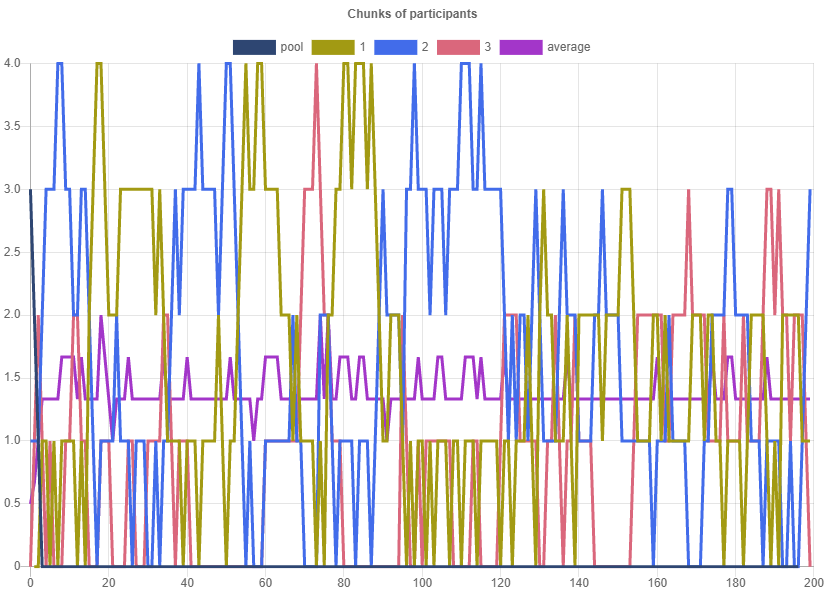
\includegraphics[width=0.8\textwidth]{media/simulation-chunks.PNG}
\end{figure}

Figures \ref{figure:simulation-converge-balance} and \ref{figure:simulation-converge-chunks} are the results of a simulation with three participants, six chunks, and was allowed to run to completion (based on the discount factor and reward threshold). Figure \ref{figure:simulation-converge-balance} shows an ideal situation in which despite varying degrees of growth, the final trend is towards the average. It shows that as participants purchase from one another, they may still have chunks in reserve, accumulating rewards passively as they trade as they are able to consistently maintain ownership of chunks for longer. In this case, the balance is likely to converge despite differing participation probabilities as participants effectively inhibit divergence through consistent trading. It is noted that the number of rounds is less than the previous simulation. This is due to the increased number of chunks resulting in lower rewards per chunk as previously defined by \cref{equation:chunkreward}.

\begin{figure}[H]
  \centering
  \caption{Balance distribution over simulation lifespan with increased chunks}
  \label{figure:simulation-converge-balance}
  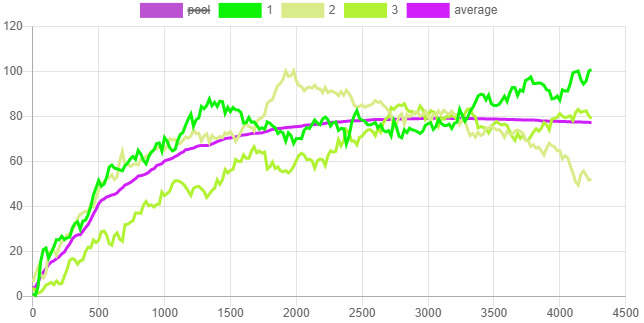
\includegraphics[width=0.8\textwidth]{media/simulation-converge-balance.PNG}
\end{figure}

Figure \ref{figure:simulation-converge-chunks} below shows the maximum difference in chunks held over the lifespan of the simulation. Over the course of the simulation, no participant held more all available chunks for longer than one round, reducing the likelihood of earning the whole balance awarded to the pool.

\begin{figure}[H]
  \centering
  \caption{Averaged chunk distribution over simulation lifespan with increased chunks}
  \label{figure:simulation-converge-chunks}
  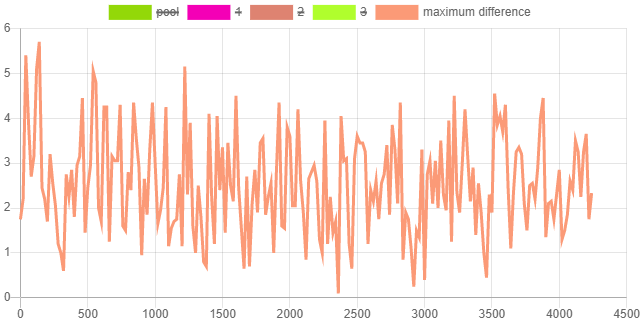
\includegraphics[width=0.8\textwidth]{media/simulation-converge-chunks.PNG}
\end{figure}

Figures \ref{figure:simulation-divergence-balance} and \ref{figure:simulation-divergence-chunks} are the results of a simulation with three participants, two chunks, and was allowed to run to completion (based on the discount factor and reward threshold). As seen in \cref{figure:simulation-divergence-balance} below, the funds appear to diverge as time goes on with one participant reaching close to an no funds. This is likely due to the fact that as the number of chunks is not enough to satisfy all participants, some participants are not able to receive a reward during some rounds and become disadvantaged due to the difference. 

\begin{figure}[H]
  \centering
  \caption{Balance distribution over simulation lifespan with decreased chunks}
  \label{figure:simulation-divergence-balance}
  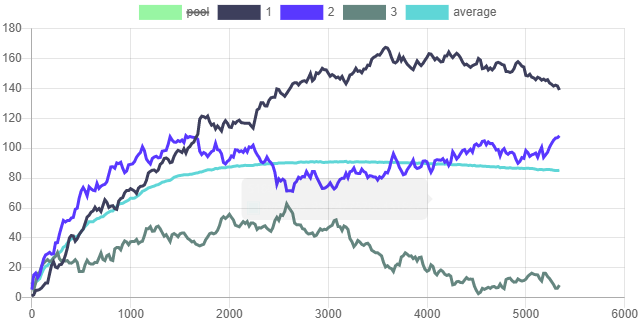
\includegraphics[width=0.8\textwidth]{media/simulation-divergence-balance.PNG}
\end{figure}

Figure \ref{figure:simulation-divergence-chunks} below shows how participant 1 was able to purchase chunks first and immediately gained an advantage with a much higher average chunk count ($\sim$0.9). Meanwhile participant 3 was had a much lower average ($\sim$0.3), leading to much slower growth. This is the least ideal instance of a game as there is a participant with a disproportionate number of chunks and is able to maintain their advantage fairly effectively.
 
\begin{figure}[H]
  \centering
  \caption{Comparison of chunk possession by participant 1 and 3 over simulation lifespan with decreased chunks}
  \label{figure:simulation-divergence-chunks}
  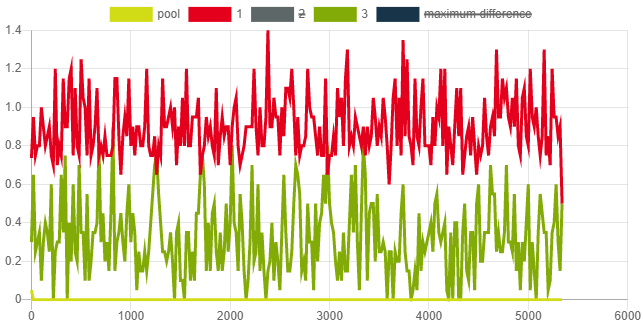
\includegraphics[width=0.8\textwidth]{media/simulation-divergence-chunks.PNG}
\end{figure}

In general, it can be seen that the ratio of chunks to participants may play a significant role in balancing the ease of achieving equilibrium. Despite the possibilities of significant losses, it is also possible to achieve a fairly distributed game if there exists the opportunity for participants to maintain possession of chunks across rounds.